\documentclass[11pt]{amsart}
\usepackage[T1]{fontenc}

\usepackage[colorlinks = true, linkcolor = black, citecolor = black, final]{hyperref}
\usepackage[left = 1.5cm, right = 1.5cm, top = 1.6cm, bottom = 1.6cm]{geometry}
\linespread{1.08}
\setlength{\parindent}{0pt}
\setlength{\parskip}{0.5\baselineskip}

\usepackage{amsthm, amsmath, amssymb}
\usepackage{graphicx, multicol}
\usepackage{marvosym, wasysym}
\usepackage{mathtools}
\usepackage{hyperref}

\DeclarePairedDelimiter{\norm}{\lVert}{\rVert}


% Acá están las líneas que cambian el estilo del texto y las ecuaciones:
%----------------------------------------------
\usepackage[noamssymbols]{newpxmath}
\usepackage{newpxtext}
%----------------------------------------------

% Cosas necesarias para que funcione Tikz:
%----------------------------------------------
\usepackage{tikz}
\usetikzlibrary{arrows,intersections}
\usetikzlibrary{angles,quotes}
\usetikzlibrary{arrows.meta}
%----------------------------------------------

\newcommand{\ds}{\displaystyle}
\DeclareMathOperator{\sech}{sech}

\pagestyle{empty}

\begin{document}

\thispagestyle{empty}

{\scshape FISI - 4405} \hfill {\scshape \Large Mecánica Analítica} \hfill {Proyecto \#1 - Thomas A. Hernández\scshape }
 
\smallskip

\hrule

\medskip

\begin{center}

{\scshape \Large \textbf{Sistema de dos ruedas bajo un potencial externo}}

\end{center}

\medskip

Este proyecto se enfoca en el estudio del sistema de la {\scshape Figure~\ref{fig:sistema}}, formado por dos ruedas idénticas de radio $a$ y masa $m$, unidas rígidamente por un eje de longitud $2b$ y masa $M$ que las mantiene paralelas sin inclinarse de la vertical. El conjunto se mueve sobre un plano horizontal fijo, con las ruedas rodando sin deslizar sobre el plano. El sistema está sujeto a un potencial externo arbitrario $V(x,y)$ que actúa únicamente sobre el centro de masa, el cual se encuentra localizado en el punto medio del eje.

\begin{figure}[h]
    \centering
    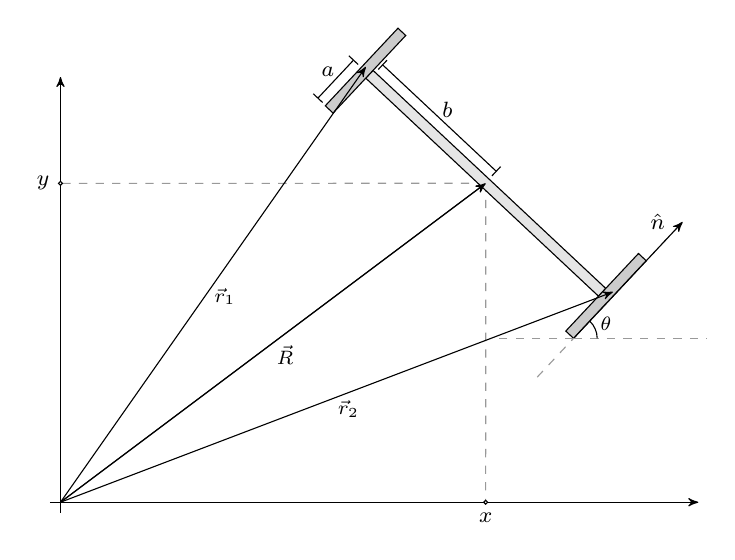
\begin{tikzpicture}[scale = 1.35, >=stealth', dot/.style = {draw, fill = white, circle, inner sep = 0pt, minimum size = 4pt}]
    % Coordenadas del punto de contacto del vector de posición del centro de masa.
    \pgfmathsetmacro{\xO}{4}
    \pgfmathsetmacro{\yO}{3}
    \pgfmathsetmacro{\angR}{atan2(\yO,\xO}
    \pgfmathsetmacro{\ang}{80}
    % Longitudes de la barra y las ruedas.
    \pgfmathsetmacro{\barO}{3}
    \pgfmathsetmacro{\wheelsO}{1.0}

    % Cambio el estilo del punto por preferencia personal la verdad.
    \tikzset{dot/.style = {circle, draw, fill=white, inner sep=0.5pt, minimum size=0.5pt}}

    % Primero se crea el eje cartesiano:
    \coordinate (O) at (0, 0);
    \draw[->] (-0.1, 0) -- (6, 0);
    \draw[->] (0, -0.1) -- (0, 4);
    
    % Incluyo el vector de posición de este vector y le calculo su ángulo.
    \draw[->] (0, 0) -- (\xO, \yO) coordinate (R);

    \draw[dashed, black!40] (R) -- (\xO,0);
    \node[dot] (x) at (\xO, 0) {};
    \node[below = 0.5pt, font = \footnotesize] at (x) {$x$};
    
    \draw[dashed, black!40] (R) -- (0,\yO);
    \node[dot] (y) at (0, \yO) {};
    \node[left = 0.5pt, font = \footnotesize] at (y) {$y$};

    \begin{scope}[shift={(R)}, rotate =\angR - \ang]
        % Barra rígida:
        \draw[fill=gray!20] (-\barO/2, -0.05) rectangle (\barO/2, 0.05);
        \draw[|-|] (-\barO/2 + 0.025, 0.15) -- (0, 0.15) node[midway, xshift = 1mm, yshift = 1mm, font = \footnotesize] {$b$};
        % Ruedas del sistema:
        \draw[fill=gray!40] (-\barO/2, -\wheelsO/2) rectangle (-\barO/2 - 0.1, \wheelsO/2);
        \draw[|-|] (-\barO/2 - 0.2, -\wheelsO/2) -- (-\barO/2 - 0.2, 0) node[midway, xshift = -1mm, yshift = 1mm, font = \footnotesize] {$a$};
        
        \draw[fill=gray!40] (\barO/2, \wheelsO/2) rectangle (\barO/2 + 0.1, -\wheelsO/2);

        % Esquemática del eje:
        \draw[dashed, black!40] (\barO/2 + 0.1, -1.0) -- (\barO/2 + 0.1, 1.0);
        \coordinate (Pang) at (\barO/2 + 0.1, -\wheelsO/2);
        \draw[->] (Pang) -- ++ (0, \wheelsO + 0.5) coordinate (n) node[left, xshift=-1mm, font = \footnotesize] {$\hat{n}$};
    \end{scope}

    \draw[->] (0,0) -- (\xO, \yO) coordinate (R) node[midway, xshift = 1.5mm, yshift = -1.5mm, font = \scriptsize] {$\vec{R}$};

    \draw[->] (0,0) -- ({\xO - (\barO/2 + 0.15)*sin(-\angR + \ang)}, {\yO + (\barO/2)*cos(-\angR + \ang)}) node[midway, xshift = 1.5mm, yshift = -1.5mm, font = \scriptsize] {$\vec{r}_{1}$};

    \draw[->] (0,0) -- ({\xO + (\barO/2 + 0.25)*sin(-\angR + \ang)}, {\yO - (\barO/2 - 0.10)*cos(-\angR + \ang)}) node[midway, xshift = 1.5mm, yshift = -1.5mm, font = \scriptsize] {$\vec{r}_{2}$};
    
    \draw[dashed, black!40] (Pang) -- ++(1.25,0) coordinate (H);
    \draw[dashed, black!40] (Pang) -- ++(-0.75,0);
    
    \pic[draw, "$\scriptstyle \theta$", angle radius=3mm, angle eccentricity = 1.5] {angle = H--Pang--n};

\end{tikzpicture}
    \caption{Sistema a estudiar. Un conjunto de coordenadas generalizadas para el sistema es el indicado en la figura, donde $x$, $y$ son las coordenadas del centro de masa, $\theta$ el ángulo que define la orientación del eje en el plano $(x, y)$, y $\phi_{1}$, $\phi_{2}$ los ángulos de rotación de cada una de las ruedas.}~\label{fig:sistema}
\end{figure}

\smallskip

\hrule

\smallskip

Para el sistema propuesto existen un total de dos restricciones de movimiento esenciales. Las ecuaciones que surgen de estas restricciones están descritas en los siguientes puntos:

\begin{enumerate}
    \item El rodamiento sin deslizamiento que sucede en ambas ruedas da origen a dos ecuaciones:
    \begin{equation}
        \dot{\vec{r}}_{1} = a\dot\phi_{1}\hat{n} \qquad \text{y} \qquad \dot{\vec{r}}_{2} = a\dot\phi_{2}\hat{n}, ~\nonumber ~\label{condicion-1}
    \end{equation}
    donde $\vec{r}_{i}$ representa el vector de posición del punto de contacto de cada rueda con el plano $xy$, mientras que $\hat{n} = (\cos\theta, \sin\theta)$ es el vector de la dirección de desplazamiento del sistema. 

    \item Las ruedas no tienen permitido moverse en la dirección paralela a la barra que las une $\hat{\theta} = (-\sin\theta, \cos\theta)$, es decir:
    \begin{equation}
        \dot{\vec{r}}_{1} \cdot \hat{\theta} = 0 \qquad \text{y} \qquad \dot{\vec{r}}_{2} \cdot \hat{\theta} = 0. ~\nonumber ~\label{condicion-2}
    \end{equation}
\end{enumerate}

Estas restricciones dependen de los vectores que determinan los puntos de contacto de cada una de las ruedas del sistema, no del vector del centro de masa. Para escribir estos vectores en términos del vector de centro de masa $\vec{R}$ hay que tener en cuenta el vector director $\hat{\theta}$ paralelo a la barra. De esta forma:
\begin{equation}
    \vec{r}_{1} = \vec{R} + b\hat{\theta} \qquad \text{y} \qquad \vec{r}_{2} = \vec{R} - b\hat{\theta}. ~\nonumber
\end{equation}
Con estos vectores en mente, las restricciones pueden reescribirse en la siguiente forma:
\begin{equation}
    \dot{\vec{r}}_{1}  = \dot{\vec{R}} + b\dot{\hat{\theta}} = \dot{\vec{R}} - b\dot{\theta}\hat{n} = a\dot\phi_{1}\hat{n} \quad \longrightarrow \quad \boxed{(\dot{\vec{R}}\cdot\hat{n}) - b\dot{\theta} = a\dot\phi_{1}}~\label{pre-ligadura1}
\end{equation}
\begin{equation}
    \dot{\vec{r}}_{2}  = \dot{\vec{R}} - b\dot{\hat{\theta}} = \dot{\vec{R}} + b\dot{\theta}\hat{n} = a\dot\phi_{2}\hat{n} \quad \longrightarrow \quad \boxed{(\dot{\vec{R}}\cdot\hat{n}) + b\dot{\theta} = a\dot\phi_{2}}~\label{pre-ligadura2}
\end{equation}
\begin{equation}
    \dot{\vec{r}}_{\text{pc}|1}\cdot\hat{\theta}  = (\dot{\vec{R}} - b\dot{\hat{\theta}})\cdot\hat{\theta} = 0 \quad \longrightarrow \quad \boxed{(\dot{\vec{R}}\cdot\hat{\theta}) = 0}  
\end{equation}

Para analizar la dinámica del sistema de una forma más cómoda, se propone escribir todo en términos de las coordenadas generalizadas $\mathbf{q} = (x, y, \theta, \Phi, \psi)$, donde las nuevas variables angulares se escriben como:
\begin{equation}
        \Phi = \frac{1}{2}(\phi_{1} + \phi_2) \qquad y \qquad \psi = \phi_{1} - \phi_{2}, ~\nonumber
\end{equation}
correspondientes a la fase media y la diferencia de fase entre las ruedas $1$ y $2$ respectivamente. Las ligaduras pueden ser reescritas en estas nuevas variables sumando y restando las ecuaciones~\eqref{pre-ligadura1} y~\eqref{pre-ligadura2}, lo cual genera las expresiones:
\begin{equation}
    2(\vec{R}\cdot\hat{n}) = a(\dot\phi_{1} + \dot\phi_{2}) \qquad \longrightarrow \qquad \boxed{(\vec{R}\cdot\hat{n}) = a\dot\Phi} ~\nonumber
\end{equation}
\begin{equation}
   -2b\dot\theta = a(\dot\phi_{1} - \dot\phi_{2}) \qquad \longrightarrow \qquad \boxed{\dot\theta = -\frac{a}{2b}\dot\psi} ~\nonumber
\end{equation}

Recopilando los resultados anteriores, las ecuaciones de las ligaduras $f_{i}$ para este sistema son las siguientes:
\[
\left\{
\begin{aligned}
    f_{1} &= -\dot{x}\sin\theta + \dot{y}\cos\theta \\
    f_{2} &= \dot{x}\cos\theta + \dot{y}\sin\theta - a\dot{\Phi} \\
    f_{3} &= \dot{\theta} + \frac{a}{2b}\dot{\psi}
\end{aligned}
\right.
\]
donde $f_{1}$ y $f_{2}$ son ligaduras no holonómicas, dado que restringen el movimiento del sistema a una región particular del espacio de configuración, contrario a $f_3$, que es una ligadura holonómica al permitir reescribir $\psi$ en términos de $\theta$, reduciendo así los grados de libertad redundantes.

\medskip

Por otra parte, para estudiar la dinámica del sistema y ver cómo se comportan los grados de libertad, el siguiente Lagrangiano provee la información base necesaria:
\begin{equation}
    L(\mathbf{q}, \dot{\mathbf{q}}, t) = \frac{1}{2}(M + 2m)(\dot{x}^{2} + \dot{y}^{2}) + \frac{1}{2}I_{M}\dot{\theta}^{2} + \frac{1}{2}I_{m}\dot{\phi}^{2}_{1} + \frac{1}{2}I_{m}\dot{\phi}^{2}_{2} - V(x, y). ~\nonumber
\end{equation}
Para reescribir en términos de $\dot\Phi$ es necesario escribir la suma de cuadrados entre $\dot\phi_{1}$ y $\dot\phi_{2}$ en términos de $\dot\Phi$ y $\dot\psi$, para luego eliminar $\dot\psi$ usando $f_{3}$, de modo que:
\begin{equation}
    \dot\phi_{1}^{2} + \dot\phi_{2}^{2} = \frac{1}{2}\left[(2\dot\Phi)^{2} + \dot\psi^{2}\right] = \frac{1}{2}\left[(2\dot\Phi)^{2} + \left(\frac{2b}{1}\right)^{2}\dot\theta^{2}\right].~\nonumber
\end{equation}
Reescribiendo el Lagrangiano\footnote{Para el paso a paso explícito de todos los procesos, revisar el archivo PDF anexado como material suplementario en el repositorio de \href{https://github.com/ThomAnkhe/Proyectos_Mecanica_Analitica/tree/main/Proyecto_1}{GitHub}.}, su expresión resulta en:
\begin{equation}
    L(\mathbf{q}, \dot{\mathbf{q}}, t) = \frac{1}{2}M_{T}(\dot{x}^{2} + \dot{y}^{2}) + \frac{1}{2}I_{T}\dot{\theta}^{2} + I_{m}\dot{\Phi}^{2} - V(x, y),
\end{equation}
donde $M_{T} = M + 2m$ y $I_T = I_{M} + 2(b/a)^{2}I_m$. Resolviendo la cinemática con las ecuaciones de Euler Lagrange e introduciendo las ligaduras se llega al siguiente sistema de ecuaciones diferenciales de segundo orden:
\[
\left\{
\begin{aligned}
    M_{T}\ddot{x} & + \partial_{x}V = -\lambda_{1}\sin\theta + \lambda_{2}\cos\theta \\
    M_{T}\ddot{y} & + \partial_{y}V = \lambda_{1}\cos\theta + \lambda_{2}\sin\theta \\
    I_{T}\ddot\theta & = 0 \\
    I_{m}\ddot\Phi & = -a\lambda_{2}
\end{aligned}
\right.,
\]
donde la fuerza de ligadura se puede construir de la forma:
\begin{equation}
    \vec{F}_{R} = (\lambda_{1}\cos\theta - \lambda_{2}\sin\theta)\hat{x} + (\lambda_{1}\sin\theta + \lambda_{2}\cos\theta)\hat{y} \quad \longrightarrow \quad \norm{\vec{F}_{R}} = \sqrt{\lambda_{1}^{2} + \lambda_{2}^{2}}.~\nonumber
\end{equation}

La única solución que persiste, independientemente del potencial suministrado, es que el ángulo de dirección $\theta(t)$ varía linealmente con el tiempo. Para solucionar para el resto de coordenadas es necesario combinar las ligaduras $f_{1}$ y $f_{2}$ junto con las ecuaciones dinámicas para poder llegar a expresiones útiles. Dos ecuaciones importantes surgen de derivar con respecto al tiempo la ligadura $f_{i}$ para luego usar la ligadura $f_{j}$, dando lugar a las expresiones:
\begin{equation}
    \dot{f}_{1} = -\ddot{x}\sin\theta + \ddot{y}\cos\theta - (\dot{x}\cos\theta + \dot{y}\sin\theta)\dot\theta = 0 \quad \longrightarrow \quad \boxed{a\dot\Phi\dot\theta = -\ddot{x}\sin\theta + \ddot{y}\cos\theta}~\label{delta-f1}
\end{equation}
\begin{equation}
    \dot{f}_{2} = \ddot{x}\cos\theta + \ddot{y}\sin\theta + (-\dot{x}\sin\theta + \dot{y}\cos\theta)\dot\theta  - \ddot\Phi = 0 \quad \longrightarrow \quad \boxed{a\ddot\Phi = \ddot{x}\cos\theta + \ddot{y}\sin\theta}~\label{delta-f2}
\end{equation}

Usando los resultados de las ecuaciones~\eqref{delta-f1} y~\eqref{delta-f2}, junto con las ecuaciones diferenciales para $x$, $y$ y $\Phi$ se puede encontrar una solución para el multiplicador de Lagrange $\lambda_{2}$, siendo este el único necesario para desglozar la dinámica del sistema:
\begin{equation}
    \lambda_{2} = \left(1 + \frac{a^{2}M_{T}}{I_{m}}\right)^{-1}\left(\frac{\partial{V(x, y)}}{\partial{x}}\cos\theta + \frac{\partial{V(x, y)}}{\partial{y}}\sin\theta\right)~\label{lambda}
\end{equation}

La anterior afirmación está respaldada en el hecho de que, al operar (~\eqref{delta-f1}$\cdot \cos\theta -$~\eqref{delta-f2}$\cdot\sin\theta$) y (~\eqref{delta-f1}$\cdot \sin\theta +$~\eqref{delta-f2}$\cdot\cos\theta$) se llega la ecuación de rodamiento sin deslizamiento para el centro de masa:
\[\left.
\begin{aligned}
    \ddot{x} & = a(\ddot\Phi\cos\theta - \dot\Phi\sin\theta) \\
    \ddot{y} & = a(\ddot\Phi\sin\theta + \dot\Phi\cos\theta)
\end{aligned}
\right\} \quad \longrightarrow \quad \ddot{\vec{R}} = a\frac{\text{d}(\dot\Phi\cdot\hat{n})}{\text{d}t} \quad \longrightarrow \quad \boxed{\dot{\vec{R}} = a\dot\Phi\cdot\hat{n}}\]

Nótese que ahora la solución del sistema se resume en hallar $\Phi(t)$ usando la expresión para el multiplicador de Lagrange $\lambda_{2}$ y la ecuación diferencial $\ddot\Phi = -(a/I_{m})\lambda_{2}$. Luego de esto, se emplea la condición de rodamiento sin deslizamiento para el centro de masa resolviendo así para $x(t)$ y $y(t)$.
\medskip
\hrule
\medskip
\begin{center}
    {\scshape \large \textbf{¿Cómo se comporta el sistema para diferentes potenciales?}}
\end{center}

Antes de empezar a explorar potenciales, es importante tener presente que para todos los escenarios, el ángulo de la dirección de desplazamiento del sistema varía linealmente como:
\begin{equation}
    \theta(t) = \dot\theta_{0}t + \theta_{0}~\nonumber
\end{equation}

\textbf{1. Potencial Nulo:} Asumiendo que $V(x,y) = 0$, el multiplicador de Lagrange $\lambda_{2}$ se anula, dado que ambas derivadas parciales del potencial son nulas. Por este motivo, la solución de la fase media será:
\begin{equation}
    \Phi(t) = \dot\Phi_{0}t + \Phi_{0} ~\nonumber
\end{equation}
Se asumirá en este y todos los demás casos que $\Phi_{0} = 0$. Con esto presente, las soluciones para la posición se vuelven:
\[
\begin{pmatrix}
    \dot{x} \\
    \dot{y}
\end{pmatrix} 
= a\dot\Phi_{0}
\begin{pmatrix}
    \cos(\dot\theta_{0}t + \theta_{0}) \\
    \sin(\dot\theta_{0}t + \theta_{0})
\end{pmatrix}
\quad \longrightarrow \quad
\begin{pmatrix}
    x(t) \\
    y(t)
\end{pmatrix} 
= a\frac{\dot\Phi_{0}}{\dot\phi_{0}}
\begin{pmatrix}
    \sin(\dot\theta_{0}t + \theta_{0}) \\
    -\cos(\dot\theta_{0}t + \theta_{0})
\end{pmatrix} + a\frac{\dot\Phi_{0}}{\dot\theta_{0}}
\begin{pmatrix}
    -\sin(\theta_{0}) \\
    \cos(\theta_{0})
\end{pmatrix}
+
\begin{pmatrix}
    x_{0} \\
    y_{0}
\end{pmatrix}
\] 

El movimiento descrito por estas ecuaciones puede verse como órbitas circulares donde su centro depende del empuje incial $\dot\theta_{0}$ que genera el movimiento:
\begin{equation}
    (x(t) - x_{0})^{2} + (y(t) - y_{0})^{2} = \left(a\frac{\dot\Phi_{0}}{\dot\theta_{0}}\right)^{2}\left[2 - 2\cos(\dot\theta_{0}t)\right]~\nonumber
\end{equation}

\textbf{2. Potencial Lineal:} Asumiendo que $V(x,y) = -F_{0}y$, ahora el multiplicador de Lagrange $\lambda_{2}$ toma un valor diferente:
\begin{equation}
    \lambda_{2} = -\lambda{F_{0}}\sin(\dot\theta_{0}t + \theta_{0}),~\nonumber
\end{equation}
donde $\lambda$ es la constante que aparece en~\eqref{lambda}. Por ende, la fase media del sistema se integra como:
\begin{equation}
    \ddot\Phi = \frac{a\lambda{F_{0}}}{I_{m}}\sin(\dot\theta_{0}t + \theta_{0}) \quad \longrightarrow \quad \dot\Phi(t) = \frac{a\lambda{F_0}}{I_{m}\dot\theta_{0}}\left[\cos(\theta_{0}) - \cos(\dot\theta_{0}t + \theta_{0}) \right] + \dot\Phi_{0} ~\nonumber
\end{equation}
\begin{equation}
    \Phi(t) = \frac{a\lambda{F_0}}{I_{m}\dot\theta_{0}}\left[\cos(\theta_{0})t - \sin(\dot\theta_{0}t + \theta_{0}) + \sin(\theta_{0})\right] + \dot\Phi_{0}t ~\nonumber
\end{equation}
Para las posiciones se obtienen las siguientes ecuaciones diferenciales:
\[
\begin{pmatrix}
    \dot{x} \\
    \dot{y}
\end{pmatrix} = \frac{a\lambda{F_0}}{I_{m}\dot\theta_{0}}\left[\cos(\theta_{0}) - \cos(\dot\theta_{0}t + \theta_{0}) \right]
\begin{pmatrix}
    \cos(\dot\theta_{0}t + \theta_0) \\
    \sin(\dot\theta_{0}t + \theta_0)
\end{pmatrix} + \dot\Phi_{0}
\begin{pmatrix}
    1 \\
    1
\end{pmatrix},
\]
cuyas soluciones son:
\[
\begin{aligned}
x(t) & = x_0 + \dot\Phi_{0}t + \frac{a\lambda{F_0}}{I_m\dot{\theta}_0} \left[\frac{\cos(\theta_0)\sin(\dot\theta_{0}t + \theta_0)}{\dot\theta_{0}} - \frac{\sin(2(\dot\theta_{0}t + \theta_0))}{4\dot\theta_{0}} - \frac{t}{2} - \frac{\sin(2\theta_{0})}{4\dot\theta_{0}}\right], \\
    y(t) & = y_0 + \dot\Phi_0t + \frac{a\lambda F_0}{I_m\dot{\theta}_0}\left[\frac{\cos(2(\dot\theta_{0} t + \theta_0))}{4\dot{\theta}_0} - \frac{\cos(\theta_0)\cos(\dot\theta_{0}t + \theta_{0})}{\dot{\theta}_0} + \frac{\sin^{2}(\theta_{0}) + 3\cos^{2}(\theta_{0})}{4\dot\theta_{0}}
\right].
\end{aligned}
\]

\textbf{3. Potencial Armónico:} Asumiendo que $V(x,y) = k(x^{2} + y^{2})/2$, ahora el multiplicador de Lagrange $\lambda_{2}$ toma la forma:
\begin{equation}
    \lambda_{2} = \lambda{k}(x\cos(\dot\theta_{0}t + \theta_{0}) + y\sin(\dot\theta_{0}t + \theta_{0})). ~\nonumber
\end{equation}

Con este valor, la fase media del centro de masa se halla con un pequeño truco que surge de derivar dos veces con respecto al tiempo:
\begin{equation}
    \ddot{\Phi} = -\frac{a\lambda{k}}{I_m}(x\cos(\dot\theta_{0}t + \theta_{0}) + y\sin(\dot\theta_{0}t + \theta_{0}))~\nonumber
\end{equation}
\begin{equation}
    \dddot\Phi(t) = -\frac{a\lambda{k}}{I_{m}}\left[(\dot{x}\cos(\dot\theta_{0}t + \theta_{0}) + \dot{y}\sin(\dot\theta_{0}t + \theta_{0})) + \dot\theta_{0}(-x\sin(\dot\theta_{0}t + \theta_{0}) + y\cos(\dot\theta_{0}t + \theta_{0}))\right]
\end{equation}
El primer paréntesis está relacionado con la ligadura $f_{2}$, mientras que el segundo se relaciona con un producto punto:  
\begin{equation}
    \dddot\Phi(t) = -\frac{a\lambda{k}}{I_{m}}\left[a\dot\Phi(t) + \dot\theta_{0}(\vec{R}\cdot\hat\theta)\right] \quad \longrightarrow \quad \ddddot\Phi(t) = -\frac{a\lambda{k}}{I_{m}}\left[a\ddot\Phi(t) + \dot\theta_{0}\left((\dot{\vec{R}}\cdot\hat\theta) + (\vec{R}\cdot\dot{\hat\theta})\right)\right]
\end{equation}




\end{document}